\documentclass[12pt,a4paper]{scrartcl}

\usepackage[english]{babel}
\usepackage[utf8x]{inputenc}
\usepackage{amsmath}
\usepackage{graphicx}
\usepackage{cite}
\usepackage{hyperref}
\usepackage{url}
\usepackage{float}
\usepackage{listings}
\usepackage[colorinlistoftodos]{todonotes}

\lstset{language=R} 

% \title{Function Reactive Programming and its speed contribution to GUI}
% \subtitle{Assignement 2 - Research setup and proposal}
% \author{Bruno Rocha Pereira - 529512}

\renewcommand{\baselinestretch}{1.5}

\begin{document}
\begin{titlepage}
    \centering
    \includegraphics[width=0.30\textwidth]{VUB.png}\par\vspace{1cm}
    {\scshape\Large Methods for scientific research\par}
    \vspace{1cm}
    {\scshape\Large Assignement 3 - Inferential Statistics\par}
    \vspace{1.5cm}
    {\Large\itshape Bruno Rocha Pereira - 0529512\par}
    \vfill
\end{titlepage}

\section{Question 1}
The data file contains reaction times for 100 users using user interfaces
with blue elements and with red elements.
\subsection{Make histograms and boxplots of distributions of both colors.}
First of all, the dataset 1 from the csv file need to be loaded.
\begin{lstlisting}[frame=single]
Question1_1 <- read.csv(file = "Data/Question1_1.csv", 
    col.names = c('User','Participant', 'Interface', 'Time'), 
    sep = ",")
\end{lstlisting}

In order to do the the histograms and the boxplots, tha data need to be split into the blue and red groups.
\begin{lstlisting}[frame=single]
reds <- subset(Question1_1, Interface=="red")
blues <- subset(Question1_1, Interface=="blue")
redsTime <- reds$Time
bluesTime <- blues$Time
\end{lstlisting}
Then we plot the histogram for the red interface with :

\begin{lstlisting}[frame=single]
hist(redsTime, xlab="Reaction Time(ms)", 
    main="Search time using red interface", col="red",
    xlim=c(0,3000),ylim=c(0,35))
\end{lstlisting}
which gives this output:

\begin{figure}[H]
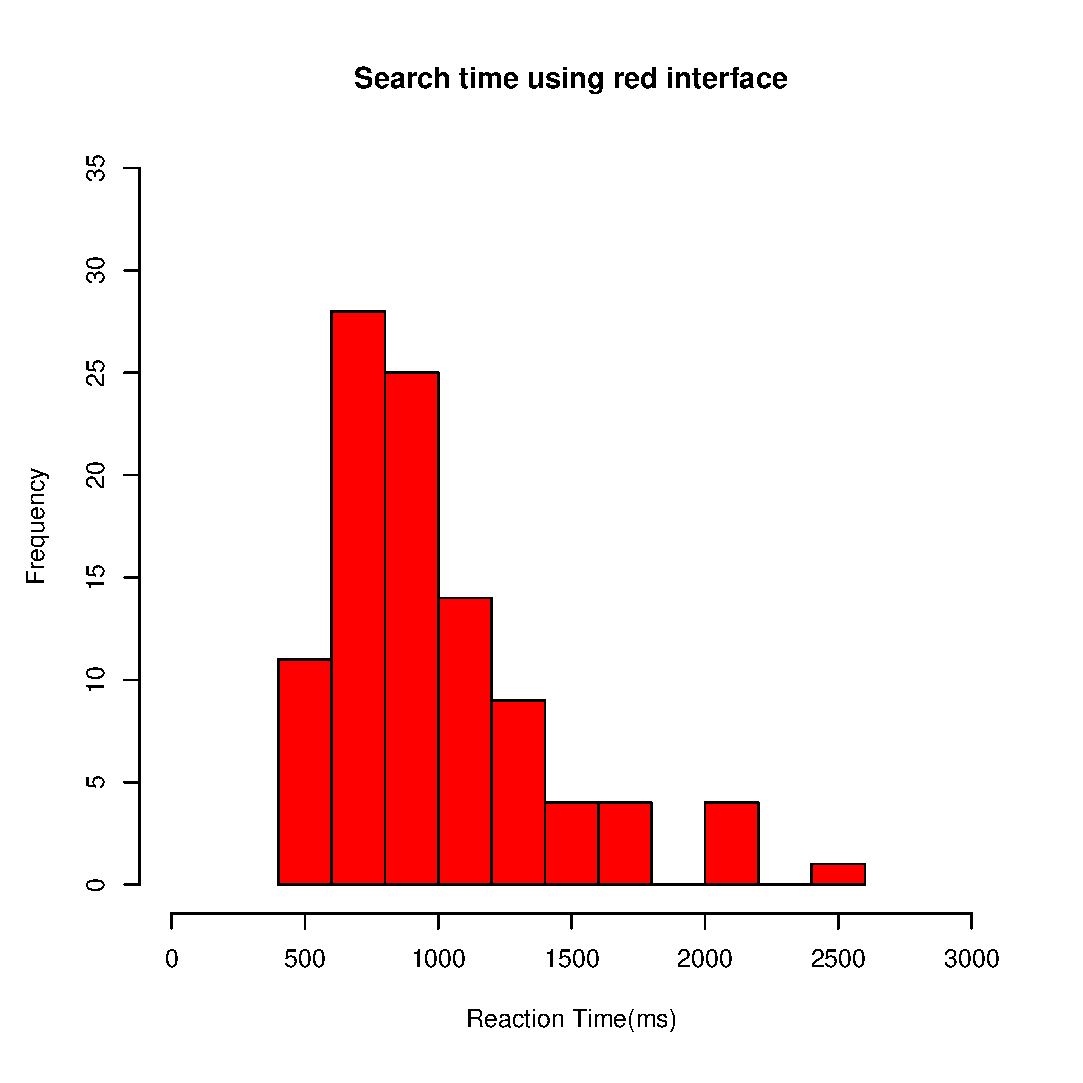
\includegraphics[scale=0.7]{Reds.eps}
\centering
\caption{Histogram for the red interface}
\end{figure}

\pagebreak
The same command is applied for the blue interface:

\begin{lstlisting}[frame=single]
hist(bluesTime, xlab="Reaction Time(ms)",
 main="Search time using blue interface", col="blue",
 xlim=c(0,3000),ylim=c(0,35))
\end{lstlisting}

\begin{figure}[H]
\includegraphics[scale=0.7]{Blues.eps}
\centering
\caption{Histogram for the blue interface}
\end{figure}

\pagebreak
The boxplot of the two distributions can also be made : 

\begin{lstlisting}[frame=single]
boxplot(redsTime,bluesTime,main="Reaction Time Boxplot", 
    names= c("Red Interface","Blue Interface"),
    col = c("red","blue"),ylab= "Reaction time (ms)")
\end{lstlisting}
\begin{figure}[H]
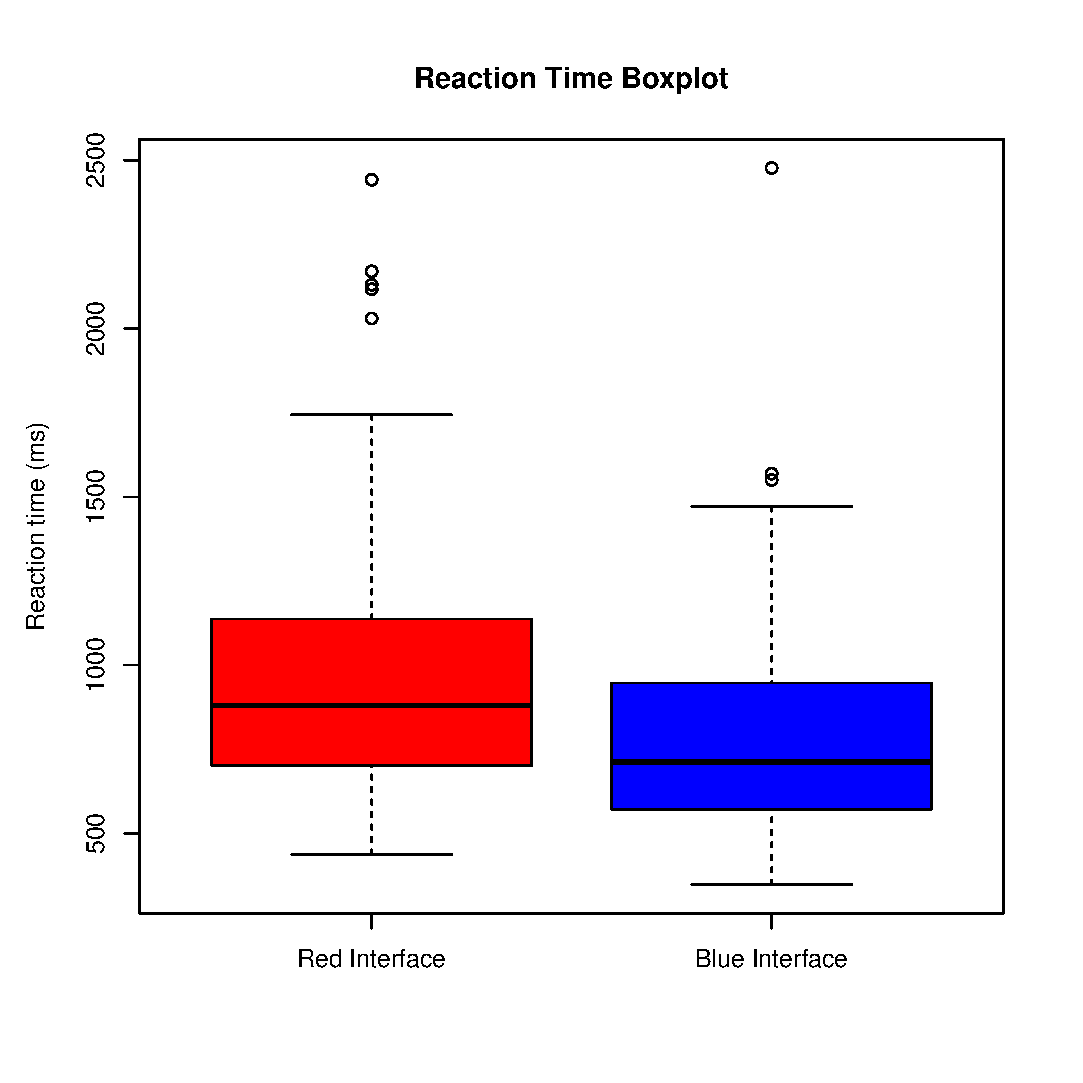
\includegraphics[scale=0.7]{Boxplot.eps}
\centering
\caption{Boxplot for the red and the blue interfaces}
\end{figure}

\subsection{Make quantile-quantile plots comparing them with the normal distribution. Does this look OK?}
The quantile-quantile plot for the red interface looks like this :

\begin{lstlisting}[frame=single]
qqnorm(redsTime, ylab = "Reaction Time (ms)", ylim = c(0, 2500))
qqline(redsTime)
\end{lstlisting}
\begin{figure}[H]
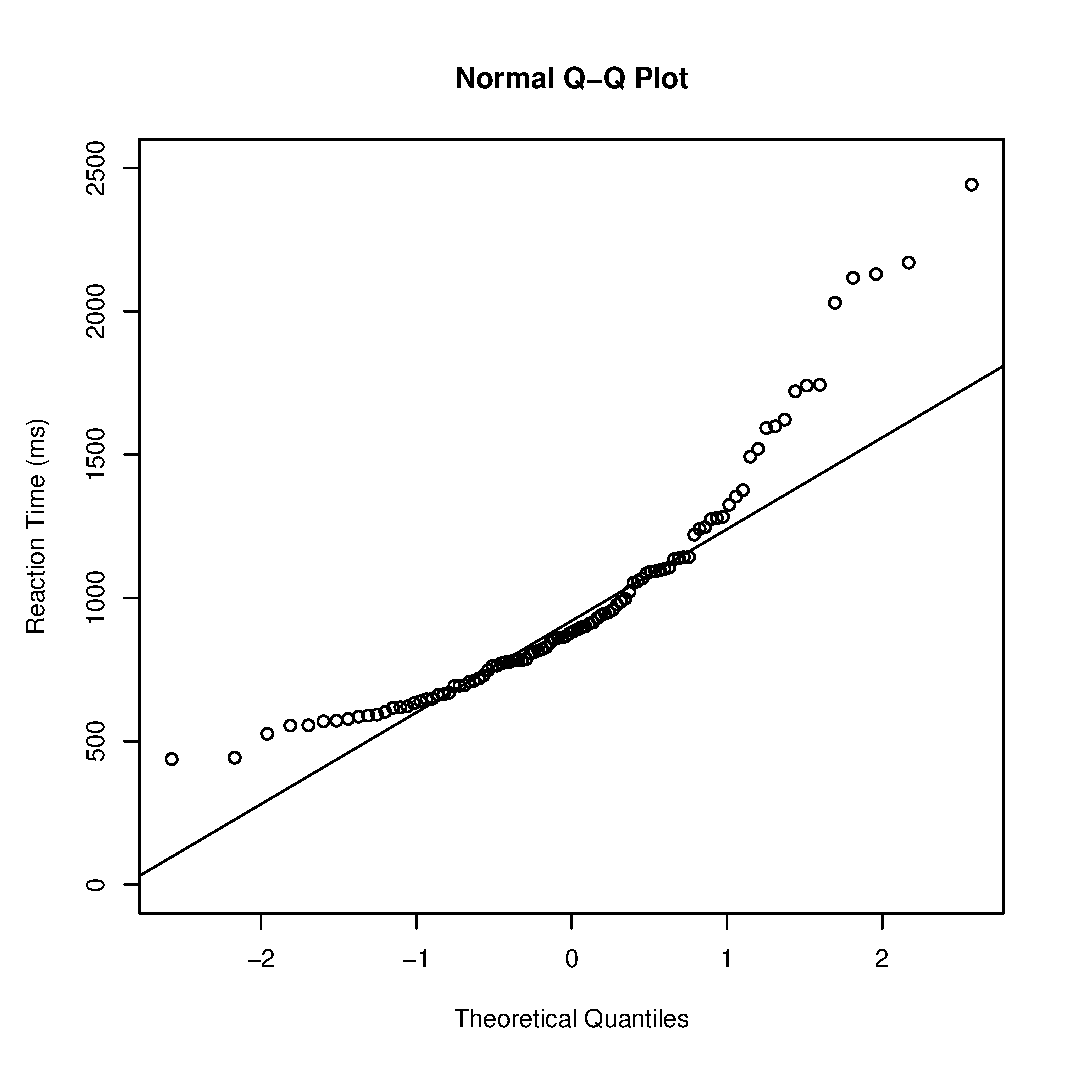
\includegraphics[scale=0.7]{QQPlotRed.eps}
\centering
\caption{Q-Q plot for the red interface}
\end{figure}

We can see on this graph that between the first and the third quantile, our distribution follows closely a normal distribution. However, this is not the case for the values below the first quantile and those above the third one, where our distribution is higher than a normal one.

On the other hand, the quantile-quantile plot for the blue interface looks like this:
\begin{lstlisting}[frame=single]
qqnorm(bluesTime, ylab = "Reaction Time (ms)", ylim = c(0, 2500))
\end{lstlisting}

\begin{lstlisting}[frame=single]
qqline(bluesTime)
\end{lstlisting}
\begin{figure}[H]
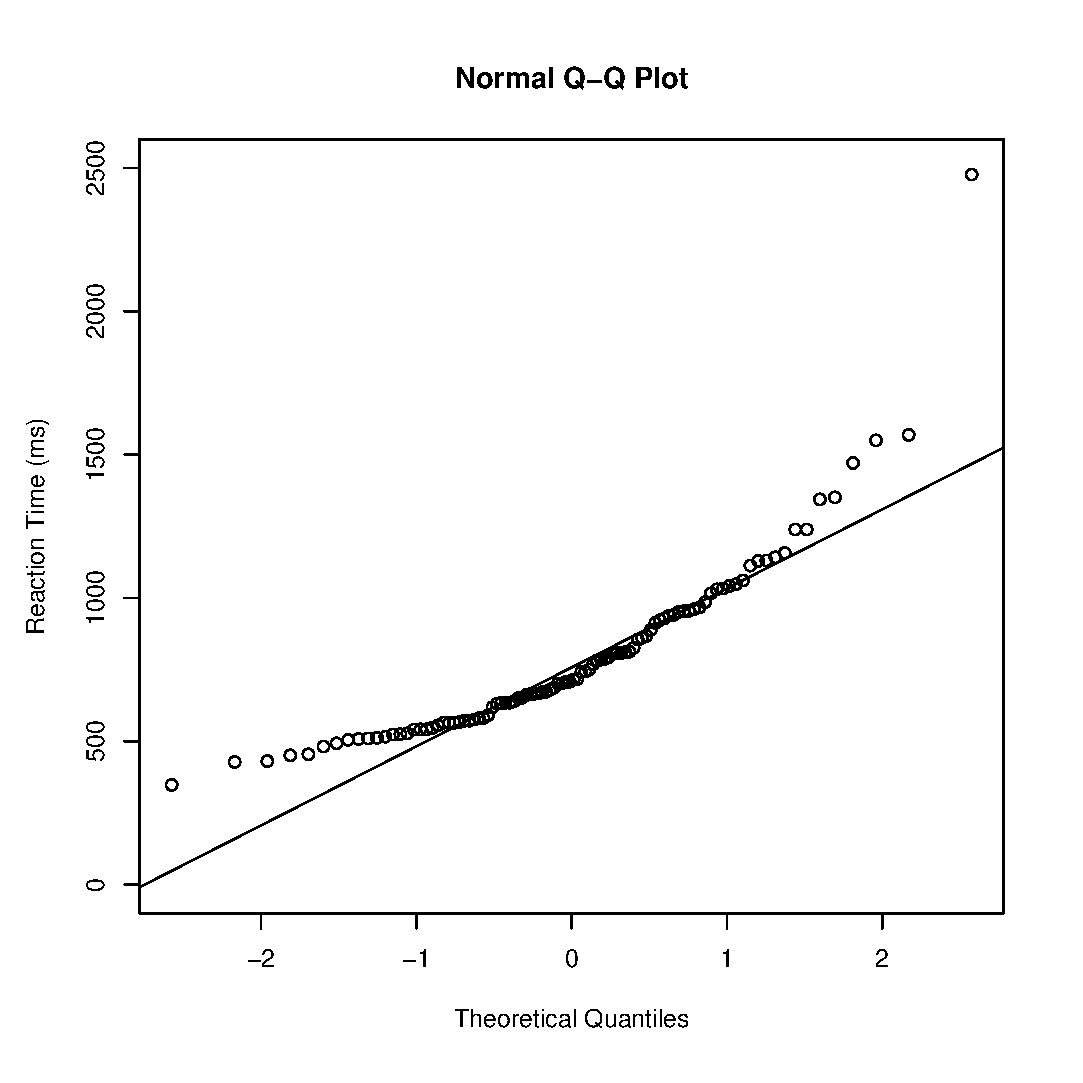
\includegraphics[scale=0.7]{QQPlotBlue.eps}
\centering
\caption{Q-Q plot for the blue interface}
\end{figure}

The distribution of the values for the blue interface looks almost like for the red one. Between the first and the third quantile, the distribution more or less follows the normal distribution, while it does not follow the normal one outside of them.

\subsection{Test whether the reaction times for the two user interfaces are different, and report the effect size}

In order to test whether the reaction times for the two different reaction times are different, we are going to make a Kruskal-Wallis test. A Kruskal-Wallis test checks if two population distributions are identical without assuming them to follow the normal distribution.\footnote{http://www.r-tutor.com/elementary-statistics/non-parametric-methods/kruskal-wallis-test}
\begin{lstlisting}[frame=single]
kruskal.test(Time~Interface, data=Question1_1)
\end{lstlisting}

gives the output
\begin{lstlisting}[frame=single, language=bash]
    Kruskal-Wallis rank sum test

data:  Time by Interface
Kruskal-Wallis chi-squared = 15.746, df = 1, p-value = 7.245e-05
\end{lstlisting}
Since the output of the Kruskal-Wallis test gives a p-value lower than 0.05, we can deduce from it that the populations have different distributions.

The effect size can be computed using a Cohen'd test.
The Cohen's d test is not built-in in R, so we have to implement it:
\begin{lstlisting}[frame=single]
cohens_d <- function(x, y) {
lx <- length(x) - 1
ly <- length(y) - 1
md <- abs(mean(x) - mean(y))
csd <- lx * var(x) + ly * var(y)
csd <- csd/(lx + ly)
csd <- sqrt(csd)
cd <- md/csd}

cohens_d(bluesTime,redsTime)
\end{lstlisting}\footnote{http://stackoverflow.com/questions/15436702/estimate-cohens-d-for-effect-size}

Using it, we get the result : effect size = 0.5394272
Since the value is close to 0.5, we can say that this is a moderate effect size.




\section{Question 2}
The data file contains numbers of bugs found in the same programming project performed by 90 different students, each one of which used either C++, C or Scheme.

First of all, the dataset 3 is imported and the data are separated by language 
\begin{lstlisting}[frame=single]

Question2_3 <- read.csv(file = "Data/Question2_3.csv",col.names = c('User', 'Language', 'Bugs'), sep = ",")
subsc <- subset(Question2_3, Language=="C")
subscpp <- subset(Question2_3, Language=="C++")
subssch <- subset(Question2_3, Language=="Scheme")
\end{lstlisting}


\subsection{Investigate whether there are significant differences between these groups, and figure out which groups are significantly different. Make sure you test the assumptions of the test you are using.}
In order to detect if there are significant differences between the groups we can use the ANOVA test, which consists of an analysis of the variances.
To see if we can use Anova, there are 3 conditions:
\begin{itemize}
\item{Variables have to be independent}
\item{Variances have to be homogeneous}
In order to prove the homogeneity of the variances, we are using the Bartlett's test.
\begin{lstlisting}[frame=single]
bartlett.test(Question2_3$Bugs,Question2_3$Language)
\end{lstlisting}
which gives Bartlett's K-squared = 0.9677, df = 2, p-value = 0.6164 

We can see that the p-value is high. We can then conclude that the variances are homogeneous.
\item{Distributions have to be normal}
In order to check the normality of the distributions, we are using the Shapiro–Wilk test on every subset.
\begin{lstlisting}[frame=single]
shapiro.test(subssch$Bugs)
    Shapiro-Wilk normality test

data:  subssch$Bugs
W = 0.9833, p-value = 0.9048

> shapiro.test(subsc$Bugs)
    Shapiro-Wilk normality test

data:  subsc$Bugs
W = 0.96691, p-value = 0.4583

> shapiro.test(subscpp$Bugs)
    Shapiro-Wilk normality test

data:  subscpp$Bugs
W = 0.98109, p-value = 0.8538
\end{lstlisting}
The null-hypothesis of the Shapiro-Wilk test test is that the population is normally distributed.
Since all of the p-values are > 0.05, we can deduce that the null-hypothesis cannot be rejected and that the distributions are normal.
\end{itemize}

We can then apply Anova to compare the variances. In order to do so, we create a model:
\begin{lstlisting}[frame=single]
labels <- gl( 3, 30 )
mymodel <- aov( Question2_3$Bugs~labels )

\end{lstlisting}
And then apply Anova on our model:
\begin{lstlisting}[frame=single]
> anova(mymodel)
Analysis of Variance Table

Response: Question2_3$Bugs
          Df Sum Sq Mean Sq F value    Pr(>F)    
labels     2  42465 21232.7  60.512 < 2.2e-16 ***
Residuals 87  30527   350.9                      
---
Signif. codes:  0 '***' 0.001 '**' 0.01 '*' 0.05 '.' 0.1 ' ' 1
\end{lstlisting}
From these results, we can extract 2 things:
\begin{itemize}
\item{The p-value is very low (2.2e-16) $\rightarrow$  0}
\item{F(2.87) = 60.512}
\end{itemize}

\pagebreak
The Anova method tells us that there is a difference but we still can't determine which groups are different. In order to determine the different pairs, we have to make a TukeyHSD test.

\begin{lstlisting}[frame=single]
> TukeyHSD(mymodel)
  Tukey multiple comparisons of means
    95% family-wise confidence level

Fit: aov(formula = Question2_3$Bugs ~ labels)

$labels
         diff       lwr      upr     p adj
2-1  2.766667 -8.766012 14.29935 0.8353479
3-1 47.400000 35.867322 58.93268 0.0000000
3-2 44.633333 33.100655 56.16601 0.0000000
\end{lstlisting}
In the output, group 1 corresponds to language C, group 2 is the Scheme language and the third one is C++.

All these tests lead to the conclusion that there is a signifant difference between C++ and the two other languages.

\subsection{Assuming a normal distribution, and aiming for a power of 0.8 and a p-value of 0.05, how large would your sample need to be to know whether there is a significant difference between the number of bugs in C and Scheme?}

In order to determine the sample size, we need to conduct a power t-test. The power t-test need the effect size, so we first compute the Cohen's d test to get it.

\begin{lstlisting}[frame=single]
c <- cohens_d(subsc$Bugs,subssch$Bugs)
\end{lstlisting}

When we have the effect size, we can apply the power t-test with it.
\begin{lstlisting}[frame=single]
power.t.test( n = NULL, d = c, sig.level = 0.05, 
    power = 0.8, sd = 1)

     Two-sample t test power calculation 

              n = 689.8112
          delta = 0.1509582 
             sd = 1
      sig.level = 0.05
          power = 0.8
    alternative = two.sided

NOTE: n is number in *each* group
\end{lstlisting}
This test gives us the sample size required to know there is a significant difference between the number of bugs in C and Scheme, which is 689 individuals. This high number can be explained by how close the distributions are.


\section{Question 3}
The data file contains information about participants using an interactive training tool to improve their programming skills. It contains their age, the number of hours they spent training and whether they passed the final test (0 indicates failure, 1 indicates success).

\begin{lstlisting}[frame=single]
Question3_1 <- read.csv(file = "Data/Question3_1.csv",
    col.names = c('Userid', 'Age', 'Training', 'Passed'), 
    sep = ",")
\end{lstlisting}
\subsection{Investigate whether the number of hours has predictive value for passing the test or not (in other words, does training longer improve performance?). Carefully explain your method.}
We are going to use here a model to fit the generalized linear symbols to find the correlation between hours of study and the fact that the student passed or not.
\begin{lstlisting}[frame=single]
model <- glm(formula = Question3_1$Passed~Question3_1$Training,
    family = binomial)
plot(Question3_1$Training, Question3_1$Passed, 
    xlab = "Hours of Training (h)", ylab = "Passed (Boolean)", 
    main= 
    "Correlation between number of hours of study and success")
points(Question3_1$Training, model$fitted, pch = "+" , 
    col = 'red')
\end{lstlisting}
This gives the below output :
\begin{figure}[H]
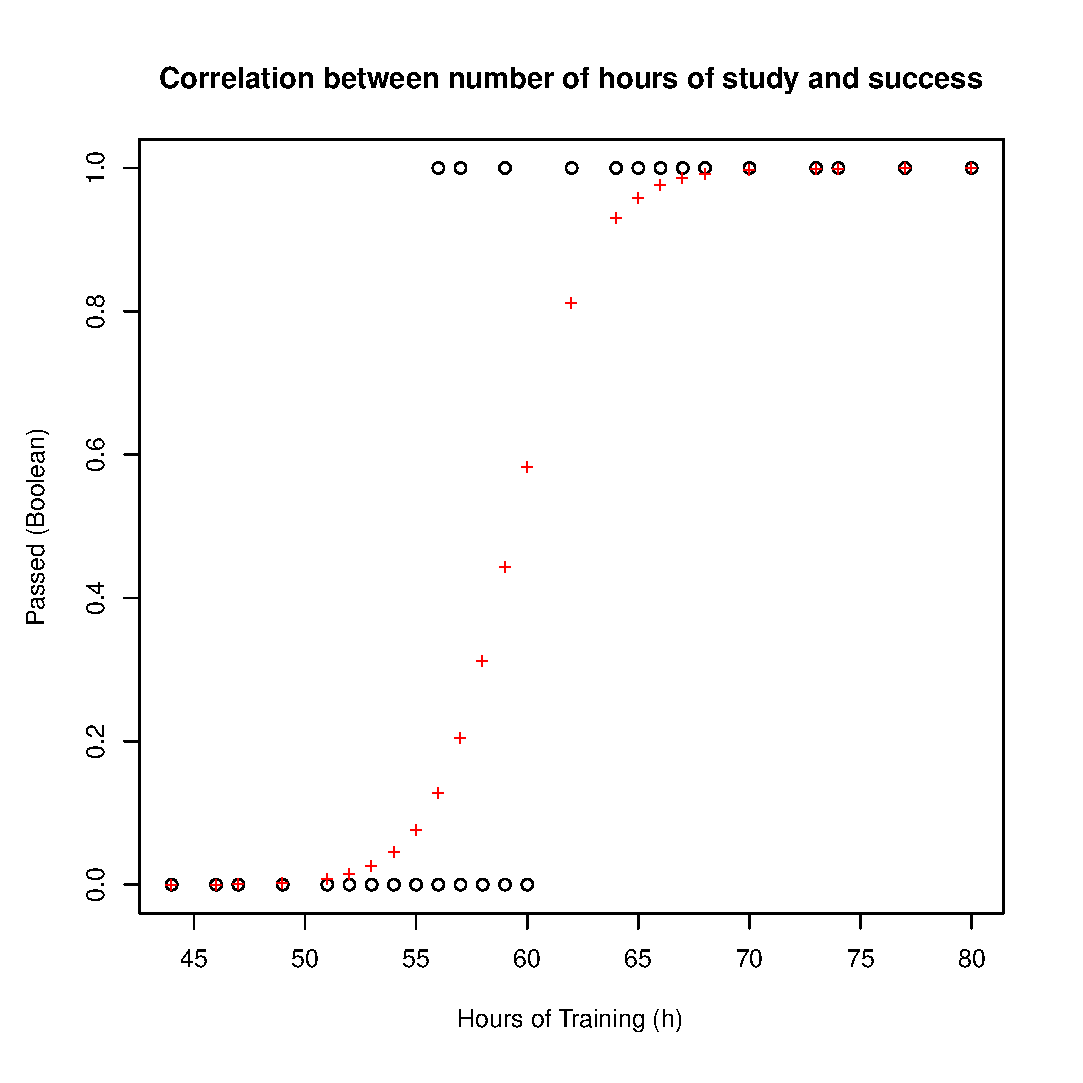
\includegraphics[scale=0.7]{model.eps}
\centering
\caption{Generalized linear model for the correlation between number of hours of training and success}
\end{figure}

The sigmoid on this graph represents the prediction of our model if there is a success or not, considering a given training duration. Two transitions can be seen around 51 and 60 hours of training. Below 50 hours of training, there is no chance of succeeding at the test, no matter how much hours of training have been involved. After that threshold, there is an exponential curve, which means that the duration of training has an impact on the success probability. The curve changes again around 60 hours of training above which we can't assume the amount of training has a significant impact on the success rate.

\subsection{Does the age of the participants have a significant influence on the outcome of the test (controlling for the effect of the number of training hours)?}
The correlation between the age and the outcome of the test will be studied controlling for the effect of the number of training hours
A cor.test wouldn't consider the controlling part of the question. We are then going to use a pcor test (from the ppcor package) with the Pearson method.

\begin{lstlisting}[frame=single]
> pcor.test(Question3_1$Age, Question3_1$Passed,
    Question3_1$Training)
    estimate   p.value  statistic  n gp  Method
1 -0.0244558 0.8675305 -0.1677107 50  1 pearson
\end{lstlisting}
On this output, we have to take a look at the estimate value. Here the estimate value is a weak negative value close to 0, which means the two variables do not vary together at all. That means there is no significant correlation between the age of the participants on the outcome of the test (controlling for the effect of the number of training hours)

\pagebreak{}
\section{Question 4}

The data file contains the number of times ICT projects with and without version management finished on time or over time.
\begin{lstlisting}[frame=single]
Question4_2 <-read.csv(file = "Data/Question4_2.csv",
    col.names=c('Type','OnTime','OverTime',sep=",")
Question4_2$Type = NULL
\end{lstlisting}


\subsection{What are the percentages of finishing on time for the two conditions?}
\begin{itemize}
\item{Percentage of finishing on time with no version control : 16.6\%}
\item{Percentage of finishing on time with version control : 37.9\%}
\end{itemize}

\subsection{Test if version management has a significant influence on whether a project runs on time or not.}

In order to test H0 = independance of variables, we are using the Fisher's Exact Test.
\begin{lstlisting}[frame=single]
> fisher.test(Question4_2,hybrid=TRUE)

    Fisher's Exact Test for Count Data

data:  Question4_2
p-value = 0.2756
alternative hypothesis: true odds ratio is not equal to 1
95 percent confidence interval:
 0.0303063 2.0386918
sample estimates:
odds ratio 
 0.3355227 
\end{lstlisting}
The p-value (0.2756) shows that there is no influence of the version control on the number of times ICT projects were finished on time or not.

\subsection{Explain why you used the test you used}
In order to test if version management has a significant influence on whether a project runs on time or not, we need a test that can be applied to contigency tables. A     
 $ \chi^{2}$ test cannot be applied to our data because one of the values is lower than 5.

\subsection{Do you find the result surprising? Can you think of a way this study could be improved?}
A bigger set of data could have been used, and the results would have been maybe different.

\end{document}
